%%% Local Variables: 
%%% coding: utf-8
%%% mode: latex
%%% TeX-engine: xetex
%%% End: 

\documentclass[hide notes,intlimits]{beamer}

\mode<presentation>
{
  \usetheme[footline]{PISMshade}
  \setbeamercovered{transparent}
}

% load packages
\usepackage{media9}
\usepackage[english]{babel}
\usepackage[multidot]{grffile}

\usepackage{tikz}
\usetikzlibrary{shapes,arrows}
\usetikzlibrary{shadows}

\definecolor{dark red}{HTML}{E41A1C}
\definecolor{dark green}{HTML}{4DAF4A}
\definecolor{dark violet}{HTML}{984EA3}
\definecolor{dark blue}{HTML}{084594}
\definecolor{dark orange}{HTML}{FF7F00}
\definecolor{light blue}{HTML}{377EB8}
\definecolor{light red}{HTML}{FB9A99}
\definecolor{light violet}{HTML}{CAB2D6}

\setbeamercolor{boxed}{fg=black,bg=light blue!25}
\graphicspath{{figures/}{../figures/}{../figures_2018_08/}}

\newenvironment{transbox}[1][]{%
\begin{tikzpicture}
\node[drop shadow,rounded corners,text width=.9\textwidth,fill=white, fill opacity=#1,text opacity=1] \bgroup
}{
\egroup;\end{tikzpicture}} 

\newenvironment{transbox-tight}{%
\begin{tikzpicture}
\node[drop shadow,rounded corners,fill=uaf yellow, fill opacity=0.75,text opacity=1] \bgroup
}{
\egroup;\end{tikzpicture}} 

\newcommand{\jl}{[\![}
\newcommand{\jr}{]\!\hskip 0.003cm ]}
\newcommand{\bpsi}{\boldsymbol{\psi}}
\newcommand{\bPsi}{\boldsymbol{\Psi}}
\newcommand{\bphi}{\boldsymbol{\phi}}
\newcommand{\bPhi}{\boldsymbol{\Phi}}
\newcommand{\bn}{\mathbf{n}}
\newcommand{\bq}{\mathbf{q}}
\newcommand{\bv}{\mathbf{v}}
\newcommand{\D}{\,\mathrm{d}}
\newcommand{\Tsnow}{T_{\text{snow}}}
\newcommand{\Hatm}{H_{\text l}^{\text{atm}}}

\newcommand{\mathtext}[1]{\mathsf{#1}}

% title page
\title[Ice sheet modeling] % (optional, use only with long paper titles)
{Do we understand uncertainties in sea-level projections?}

\author[Aschwanden] % (optional, use only with lots of authors)
{\textbf{Andy Aschwanden}, M. Truffer, D. Brinkerhoff, T. Bartholomaus}
\institute{Geophysical Institute, University of Alaska Fairbanks}

% - Give the names in the same order as the appear in the paper.
% - Use the \inst{?} command only if the authors have different
%   affiliation.

% - Use the \inst command only if there are several affiliations.
% - Keep it simple, no one is interested in your street address.

% \titlegraphic{\vskip-1.cm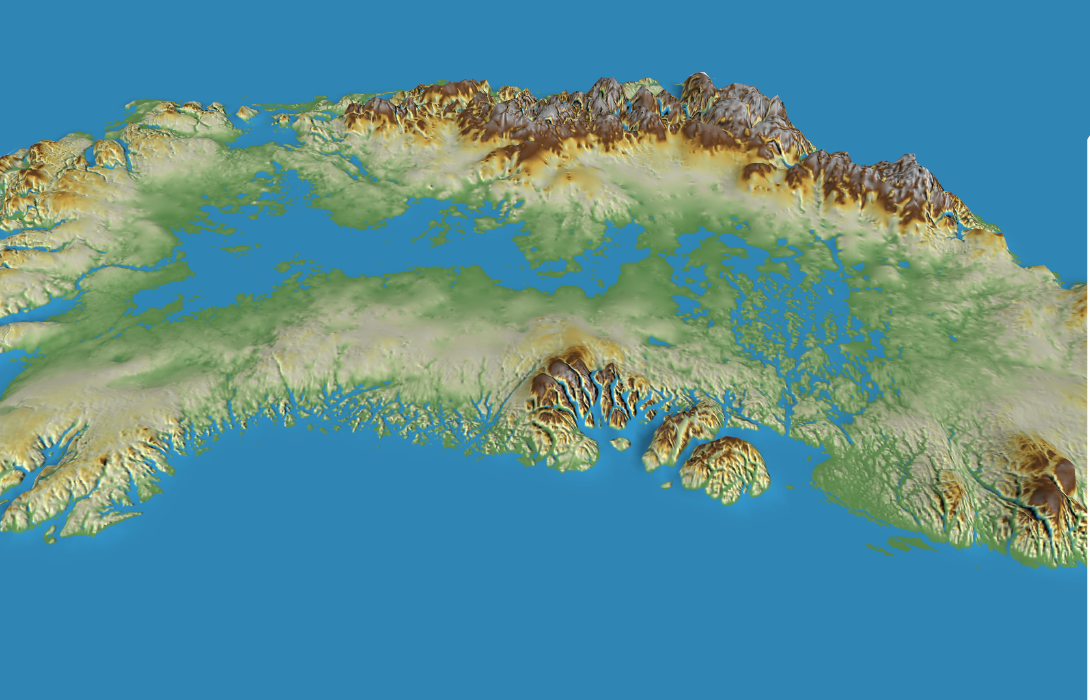
\includegraphics[height=3.5cm]{gris-green-collage-clean}}

\date{}


\subject{The Greenland Ice Sheet}

\begin{document}


\setbeamertemplate{background canvas}
  {
     \tikz{\node[inner sep=0pt,opacity=1.0] {\includegraphics[width=\paperwidth]{uaf_beamer_shade_bg}};}
} 

% insert titlepage
\begin{frame}
  \titlepage
  \note[item]{Collaboration with Martin, Doug, and Tim}
\end{frame}


%% \setbeamertemplate{background canvas}
%%   {
%%      \tikz{\node[inner sep=0pt,opacity=1] {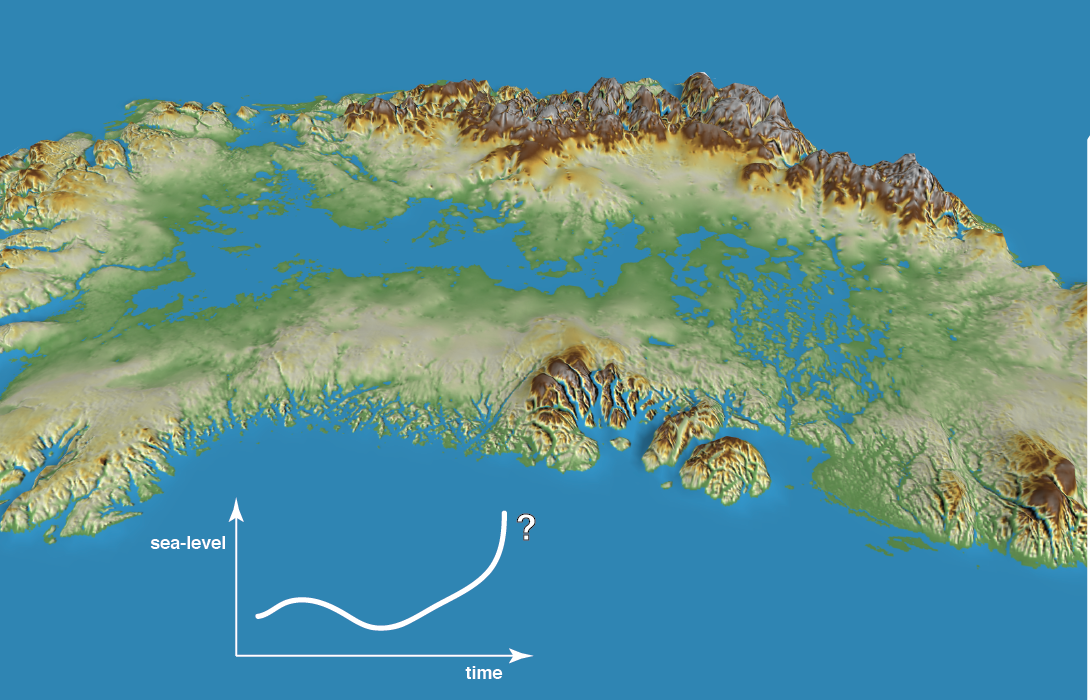
\includegraphics[height=\paperheight,width=\paperwidth]{gris-green-collage-slr}};}
%% } 


\setbeamertemplate{background canvas}
{
%
}



\begin{frame}{ISMIP6 Greenland}
  \begin{figure}
    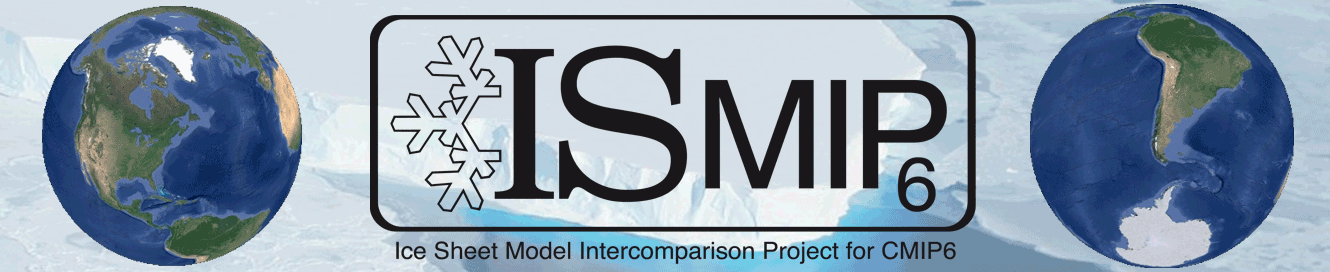
\includegraphics[width=0.9\textwidth]{ismip6_logo}
  \end{figure}
  \begin{itemize}
  \item Ice Sheet Model Intercomparison for CMIP Phase 6
  \item ISMIP6 is misleading: first such effort ever
  \item Number of modeling groups participated: 13
  \item Number of ice sheet model configurations used: 18
  \item Number of experiments: 9
  \end{itemize}
  \note[item]{}
\end{frame}

\begin{frame}{GitHub and Binder}
  \begin{figure}
    \includegraphics<1>[width=\textwidth]{ismip6-ipcc-binder}
    \includegraphics<2>[width=\textwidth]{ismip6-ipcc-binder-click}
  \end{figure}
  \note[item]{}
\end{frame}


\begin{frame}{ISMIP6}
  \begin{figure}
    \includegraphics<1>[width=\textwidth]{GIS_ismip6_projection}
    \includegraphics<2>[width=\textwidth]{GIS_ismip6_projection_stats}
  \end{figure}
  shading: 16/84th percentile
  \note[item]{}
\end{frame}


\begin{frame}{ISMIP6 + Aschwanden et al (2019)}
  \begin{figure}
    \includegraphics<1>[width=\textwidth]{GIS_ismip6_as19_projection}
  \end{figure}
  shading: 16/84th percentile
  \note[item]{}
\end{frame}

\begin{frame}{ISMIP6: Historical simulation}
  \begin{itemize}
  \item most simulations under-estimate contemporary mass loss
  \item (...and thus likley under-estimate future mass loss)
  \end{itemize}
  \begin{figure}
    \includegraphics<1>[width=\textwidth]{GIS_historical}
  \end{figure}
  \begin{itemize}
    \item ``not meant to reproduce observations''
  \end{itemize}
  \note[item]{}
\end{frame}

\begin{frame}{The dilemma}
  \begin{columns}[c]
    \begin{column}{.5\linewidth}
      \begin{itemize}
      \item ``not meant to reproduce observations''
      \item ``these are projection of 21st century mass loss''
      \end{itemize}
    \end{column}
    \begin{column}{.5\linewidth}
      \alert{$\Rightarrow$ no you can't have your cake and eat it too!!}
    \end{column}
  \end{columns}
  \note[item]{}
\end{frame}

\begin{frame}{A19 calibrated with GRACE}
  \begin{figure}
    \includegraphics<1>[width=0.85\textwidth]{sle_pdf_rcps_2100}
    \includegraphics<2>[width=0.85\textwidth]{sle_pdf_calibrated_rcps_2100}
  \end{figure}
  \begin{columns}[c]
    \begin{column}{.33\linewidth}
      \begin{itemize}
      \item 3-$\sigma$: 31 (6.3\%)
      \item 2-$\sigma$: 29 (5.9\%)
      \item 1-$\sigma$: 20 (4.1\%)
      \end{itemize}
    \end{column}
    \begin{column}{.33\linewidth}
      \begin{itemize}
      \item 3-$\sigma$: 35 (7.1\%)
      \item 2-$\sigma$: 28 (5.7\%)
      \item 1-$\sigma$: 16 (3.3\%)
      \end{itemize}
    \end{column}
    \begin{column}{.33\linewidth}
      \begin{itemize}
      \item 3-$\sigma$: 45 (9.4\%)
      \item 2-$\sigma$: 30 (6.3\%)
      \item 1-$\sigma$: 22 (4.6\%)
      \end{itemize}
    \end{column}
  \end{columns}
  
  \note[item]{}
\end{frame}


\begin{frame}{Marginal distributions}
  \begin{figure}
    \includegraphics<1>[height=\textheight]{marginal_distributions_kde}
  \end{figure}
  \note[item]{}
\end{frame}

\begin{frame}{Marginal distributions: speed calibration}
  \begin{figure}
    \includegraphics<1>[height=\textheight]{speed_emulator_parameter_posterior}
  \end{figure}
  \note[item]{}
\end{frame}


\end{document}
